\chapter{Capítulo Octavo - Desarrollo del Sistema}
Este capítulo recoge la especificación, el diseño y la implementación de TankGo, así como
el plan de pruebas y el manual de usuario. Es el núcleo técnico del proyecto y documenta
las decisiones de arquitectura, las tecnologías empleadas y el resultado final del sistema.

% ═════════════════════════════════════════════
\section{Especificación de Requisitos}
% ═════════════════════════════════════════════

\subsection{Contexto del sistema}

TankGo es una plataforma de inteligencia de datos orientada a la movilidad y la eficiencia
energética. Su propósito es transformar los datos abiertos del Geoportal de Gasolineras del
Ministerio para la Transición Ecológica~\cite{geoportal_gasolineras} en información
accionable para el conductor, añadiendo capas de valor mediante análisis histórico,
predicción de precios y recomendación geoespacial de repostaje.

El sistema actúa como intermediario entre las fuentes de datos públicos y el usuario final,
operando en un entorno cloud que permite tanto la consulta en tiempo real como el
entrenamiento y servicio de modelos de machine learning. A diferencia de un visor estático,
TankGo integra en una única plataforma la consulta de gasolineras y electrolineras, la
estimación de precios futuros y un asistente conversacional por voz para interacción en
manos libres.

\subsection{Identificación de usuarios}

El sistema contempla dos perfiles de usuario diferenciados. El \textbf{usuario no registrado}
puede acceder a las funciones de consulta pública: visualización de gasolineras y
electrolineras en mapa y tabla, detalle de cada estación y precios actuales. El
\textbf{usuario registrado} dispone, además, de la gestión de estaciones favoritas, el
acceso al histórico de precios de cada estación y las predicciones a 7 días generadas por
el modelo de machine learning.

Dentro de estos perfiles, los casos de uso más representativos son el conductor particular
que busca repostar barato en su área, el transportista profesional que planifica rutas de
larga distancia con criterios de coste, y el usuario de vehículo eléctrico que necesita
localizar puntos de recarga en ruta.

\subsection{Requisitos funcionales}

Los requisitos funcionales definen las capacidades que el sistema debe ofrecer al
usuario~\cite{sommerville2011}. La tabla~\ref{tab:rf} recoge los requisitos identificados
para TankGo.
\begin{table}[H]
  \centering
  \caption{Requisitos funcionales del sistema}
  \label{tab:rf}
  \begin{tabular}{llp{9cm}}
    \toprule
    \textbf{ID} & \textbf{Requisito} & \textbf{Descripción} \\
    \midrule
    RF-01 & Consulta de gasolineras     & El sistema muestra las estaciones de servicio cercanas a la ubicación del usuario en tabla y mapa interactivo, con detalle de precios por tipo de combustible. \\
    RF-02 & Consulta de electrolineras  & El sistema muestra los puntos de recarga eléctrica disponibles en un mapa independiente. \\
    RF-03 & Histórico de precios        & Para cada estación, el sistema permite visualizar la evolución histórica del precio de cada combustible. \\
    RF-04 & Predicción de precios       & El sistema estima el precio de combustible para los próximos 7 días en las estaciones marcadas como favoritas por el usuario. \\
    RF-05 & Gestión de favoritos        & El usuario registrado puede marcar y gestionar sus estaciones de servicio favoritas. \\
    RF-06 & Recomendación en ruta       & El sistema sugiere paradas de repostaje óptimas a lo largo de una ruta, ponderando precio y desvío. \\
    RF-07 & Asistente conversacional    & El sistema permite realizar consultas en lenguaje natural mediante voz, como localizar la gasolinera más barata en la zona. \\
    RF-08 & Autenticación de usuarios   & El sistema permite el registro e inicio de sesión mediante Google OAuth. \\
    \bottomrule
  \end{tabular}
\end{table}

\subsection{Requisitos no funcionales}

Los requisitos no funcionales establecen las propiedades de calidad del sistema, no
directamente relacionadas con las funciones que ofrece, sino con cómo las
ofrece~\cite{sommerville2011}.

\textbf{Disponibilidad (RNF-01):} Al tratarse de una plataforma de consulta en ruta, el
sistema debe garantizar un tiempo de actividad superior al 99\%, respaldado por la
infraestructura de Google Cloud Platform.

\textbf{Latencia (RNF-02):} El tiempo de respuesta de las consultas de precios y el
asistente conversacional no deben ser muy elevados, requisito crítico para garantizar
la seguridad vial en uso móvil.

\textbf{Escalabilidad (RNF-03):} La arquitectura de microservicios y el despliegue en
Cloud Run permiten escalar cada componente de forma independiente según la demanda, sin
afectar al resto del sistema.

\textbf{Usabilidad (RNF-04):} El frontend está diseñado con criterio \textit{mobile-first}
y es completamente responsivo, priorizando la experiencia en dispositivos móviles sin
renunciar a la usabilidad en escritorio.

\textbf{Seguridad (RNF-05):} Las comunicaciones se realizan sobre HTTPS, la autenticación
se gestiona mediante tokens JWT y el acceso a los microservicios internos está restringido
a través del API Gateway.

\subsection{Restricciones}

El sistema opera bajo tres restricciones principales. En primer lugar, existe una
\textbf{dependencia de fuentes externas}: los datos de gasolineras provienen de la API
pública del Ministerio para la Transición Ecológica~\cite{datosgob_carburantes}, cuya
disponibilidad y frecuencia de actualización están fuera del control del sistema. En segundo
lugar, las funciones de consulta, predicción y recomendación requieren \textbf{conectividad
activa a internet}, ya que toda la lógica reside en el backend cloud. Finalmente, el
\textbf{asistente conversacional} está diseñado para responder consultas puntuales, no para
mantener diálogos extendidos mientras se conduce, en línea con las directrices de seguridad
vial aplicables. El sistema de recomendacion de rutas tambien añade una dependecia esta fuera del control del sistema, ya que se basa en la API de Open Route Service para el cálculo de rutas y distancias.

% ═════════════════════════════════════════════
\section{Diseño del Sistema}
% ═════════════════════════════════════════════

\subsection{Alternativas exploradas y decisiones tecnológicas}
Las decisiones tecnológicas de TankGo responden a criterios de adecuación funcional,
rendimiento en entornos cloud y familiaridad del equipo de desarrollo. A continuación se
justifican las elecciones más relevantes.

Para el \textbf{API Gateway} se han evaluado opciones como Kong, AWS API Gateway y soluciones
basadas en Nginx. Se ha optado por \textbf{Hono sobre Node.js} por su bajo consumo de recursos,
su rendimiento en entornos serverless y su sintaxis próxima a Express, lo que simplificó la
curva de aprendizaje~\cite{hono}. Hono permite implementar enrutamiento, middleware de
autenticación y políticas CORS con un código mínimo y muy legible.

Para los \textbf{microservicios de dominio} se han utilizado dos tecnologías según el
lenguaje más adecuado para cada caso. El servicio de usuarios se implementó con
\textbf{Fastify (Node.js)}, un framework orientado al alto rendimiento con una gestión
eficiente del esquema de validación. Los servicios de gasolineras,
recomendación y predicción se implementaron con \textbf{FastAPI (Python)}, elección
motivada por la integración nativa con el ecosistema de machine learning de Python
(scikit-learn, LightGBM, pandas) y su capacidad para generar documentación OpenAPI
automáticamente.

Para el \textbf{frontend} se ha optado por \textbf{React con TypeScript y Vite}, combinación
que ofrece tipado estático, tiempos de compilación reducidos y un ecosistema de componentes
amplio. La aplicación está construida como \textit{Progressive Web App} (PWA), lo que
permite su uso en dispositivos móviles con comportamiento nativo.

La \textbf{base de datos} es PostgreSQL, desplegada en Neon Cloud \cite{neon_cloud}. Se ha elegido PostgreSQL por su solidez,
soporte de extensiones geoespaciales y compatibilidad con los ORM uilizados en ambos
stacks tecnológicos.


\subsection{Arquitectura general}

TankGo sigue una \textbf{arquitectura de microservicios} en la que cada funcionalidad
principal del sistema se encapsula en un servicio independiente con su propia lógica y
despliegue. Los servicios se comunican entre sí a través de una capa de API Gateway que
actúa como punto de entrada único para el cliente.

La arquitectura se organiza en cuatro niveles. El \textbf{cliente} es la aplicación React
PWA que el usuario final consume desde el navegador o dispositivo móvil. El
\textbf{API Gateway} (Hono) recibe todas las peticiones del cliente, gestiona la
autenticación y las enruta hacia el microservicio correspondiente. La \textbf{capa de
servicios} agrupa los cinco microservicios del dominio: usuarios, gasolineras,
electrolineras, recomendación y predicción. Finalmente, la \textbf{capa de persistencia}
centraliza el almacenamiento en PostgreSQL, accesible desde cada servicio según sus
necesidades.

\begin{figure}[H]
  \centering
  %\includegraphics[width=0.85\textwidth]{figures/arquitectura.png}
  \caption{Diagrama de arquitectura general de TankGo}
  \label{fig:arquitectura}
\end{figure}

\subsection{Diseño lógico y físico}
Desde el punto de vista \textbf{lógico}, el sistema se estructura en torno a cinco
entidades de dominio principales: \textit{Estación de servicio}, \textit{Precio},
\textit{Usuario}, \textit{Favorito} y \textit{Predicción}. Las estaciones concentran la
información geolocalizada de cada gasolinera o electrolinera; los precios registran tanto
el valor actual como el histórico asociado a cada estación y tipo de combustible; los
usuarios encapsulan la identidad y preferencias de cada cuenta; los favoritos modelan la
relación entre usuario y estación; y las predicciones almacenan las estimaciones generadas
por el modelo de machine learning para su consulta posterior.

Desde el punto de vista \textbf{físico}, cada microservicio se despliega como un contenedor
Docker independiente. En producción, los servicios corren en \textbf{Google Cloud Run},
que gestiona el escalado automático en función de la demanda. La base de datos reside en
\textbf{Neon Tech} (PostgreSQL), y los artefactos de los modelos de machine learning se
almacenan en \textbf{Cloud Storage}. El tráfico externo entra exclusivamente por el API
Gateway, que es el único componente con URL pública expuesta.

\subsection{Modelo de datos}

El esquema de base de datos de TankGo se compone de cinco tablas principales cuyo diseño
refleja directamente el dominio del sistema.

La tabla \texttt{gasolineras} es la entidad central del modelo. Almacena la información
estática y los precios actuales de cada estación de servicio, identificada de forma única
mediante el campo \texttt{ideess} (identificador oficial del Ministerio). Incluye datos de
localización (municipio, provincia, dirección, coordenadas y geometría PostGIS), horario
en formato estructurado (\texttt{horario\_parsed} en JSONB) y los precios actuales de cada
tipo de combustible: Gasolina 95 E5, 98 E5, Gasóleo A, Gasóleo B, Gasóleo Premium,
Gasolina 95 Premium y Diésel Renovable.

La tabla \texttt{precios\_historicos} registra la evolución temporal de los precios por
estación. Cada registro asocia un \texttt{ideess} con una fecha y los precios de los
distintos combustibles en ese momento, lo que permite construir series temporales para el
análisis histórico y el entrenamiento del modelo de predicción.

La tabla \texttt{prediction\_forecasts} almacena las estimaciones generadas por el modelo
LightGBM. Su clave primaria es compuesta: \texttt{ideess}, \texttt{fuel},
\texttt{forecast\_date} y \texttt{run\_date}, lo que permite distinguir predicciones para
diferentes combustibles, horizontes temporales y ejecuciones del modelo. Cada registro
incluye el precio predicho y los márgenes de confianza inferior y superior.

La tabla \texttt{users} gestiona las cuentas de usuario, incluyendo autenticación
tradicional mediante \texttt{password\_hash} y autenticación federada mediante
\texttt{google\_id} (OAuth). Almacena también las preferencias del usuario como el
combustible favorito, el modelo de coche y el tipo de combustible del vehículo.

La tabla \texttt{user\_favorites} modela la relación entre usuarios y estaciones,
permitiendo que cada usuario registre sus gasolineras favoritas. Referencia mediante
claves foráneas tanto a \texttt{users.id} como a \texttt{gasolineras.ideess}.

Las dependencias entre tablas son las siguientes: \texttt{precios\_historicos} y
\texttt{user\_favorites} referencian \texttt{gasolineras} a través de \texttt{ideess};
\texttt{prediction\_forecasts} referencia igualmente a \texttt{gasolineras}; y
\texttt{user\_favorites} referencia a \texttt{users} mediante \texttt{user\_id}. El
diagrama entidad-relación de la figura~\ref{fig:er} ilustra estas relaciones.

\begin{figure}[H]
  \centering
  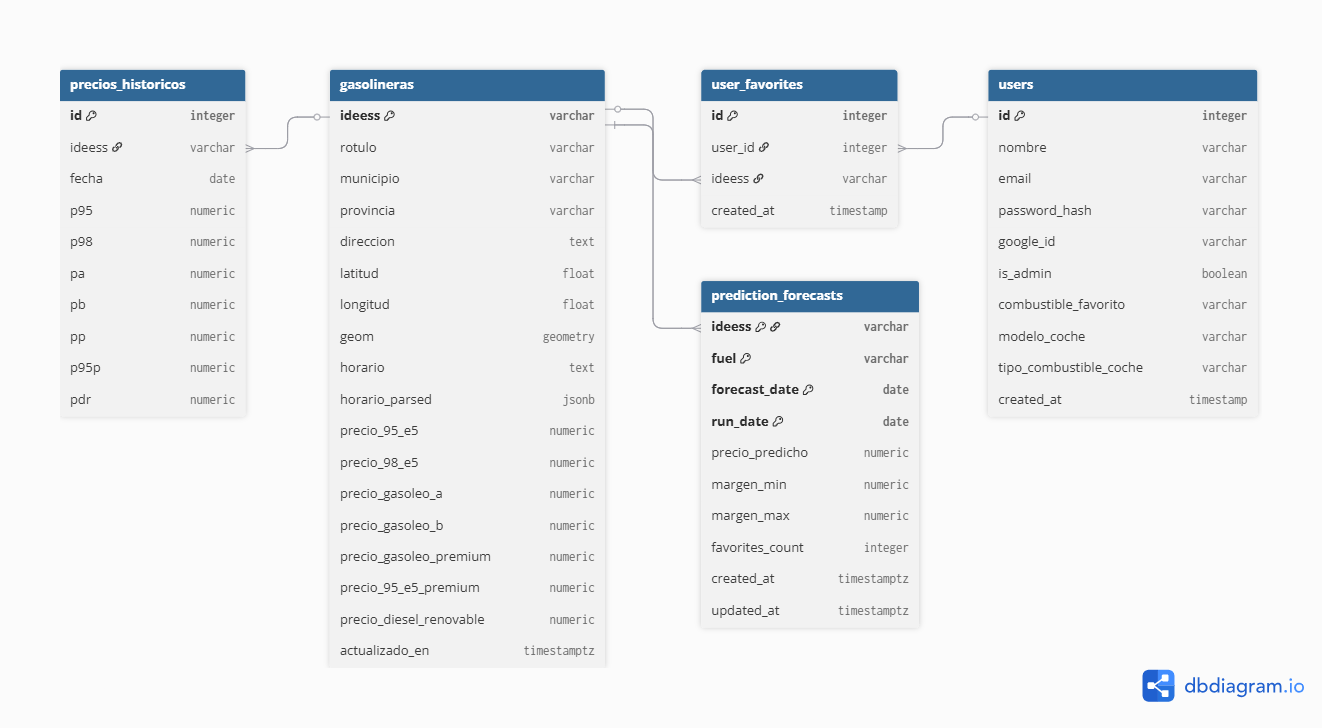
\includegraphics[width=0.85\textwidth]{imgs/entidad-relacion.png}
  \caption{Modelo entidad-relación del sistema}
  \label{fig:er}
\end{figure}

\subsection{Diagramas UML}

El diagrama de casos de uso recoge las interacciones entre los actores del sistema y sus
funcionalidades. El \textit{usuario no registrado} puede visualizar gasolineras en mapa y
tabla, consultar el mapa de electrolineras y registrarse o iniciar sesión. El
\textit{usuario registrado} extiende esas capacidades con acceso a la tabla de
electrolineras, la planificación de rutas con recomendación de repostaje, el asistente
conversacional, la predicción de precios a 7 días, la gestión de favoritos y el histórico
de precios. El sistema interactúa además con tres actores externos: la API del Ministerio
(MITECO) para la sincronización de precios, la Reve API para los puntos de recarga
eléctrica, y OpenRouteService para el cálculo de rutas.

\begin{figure}[H]
  \centering
  %\includegraphics[width=0.85\textwidth]{imgs/casos-uso.png}
  \caption{Diagrama de casos de uso del sistema}
  \label{fig:casos_uso}
\end{figure}

El diagrama de secuencia de la figura~\ref{fig:secuencia_consulta} ilustra el flujo de
consulta de gasolineras cercanas: el usuario activa la geolocalización, el frontend envía
la petición al API Gateway, este la enruta al servicio de gasolineras, que ejecuta una
consulta geoespacial sobre PostgreSQL mediante PostGIS y devuelve el listado de estaciones
con sus precios actuales para su renderizado en tabla y mapa.

\begin{figure}[H]
  \centering
  %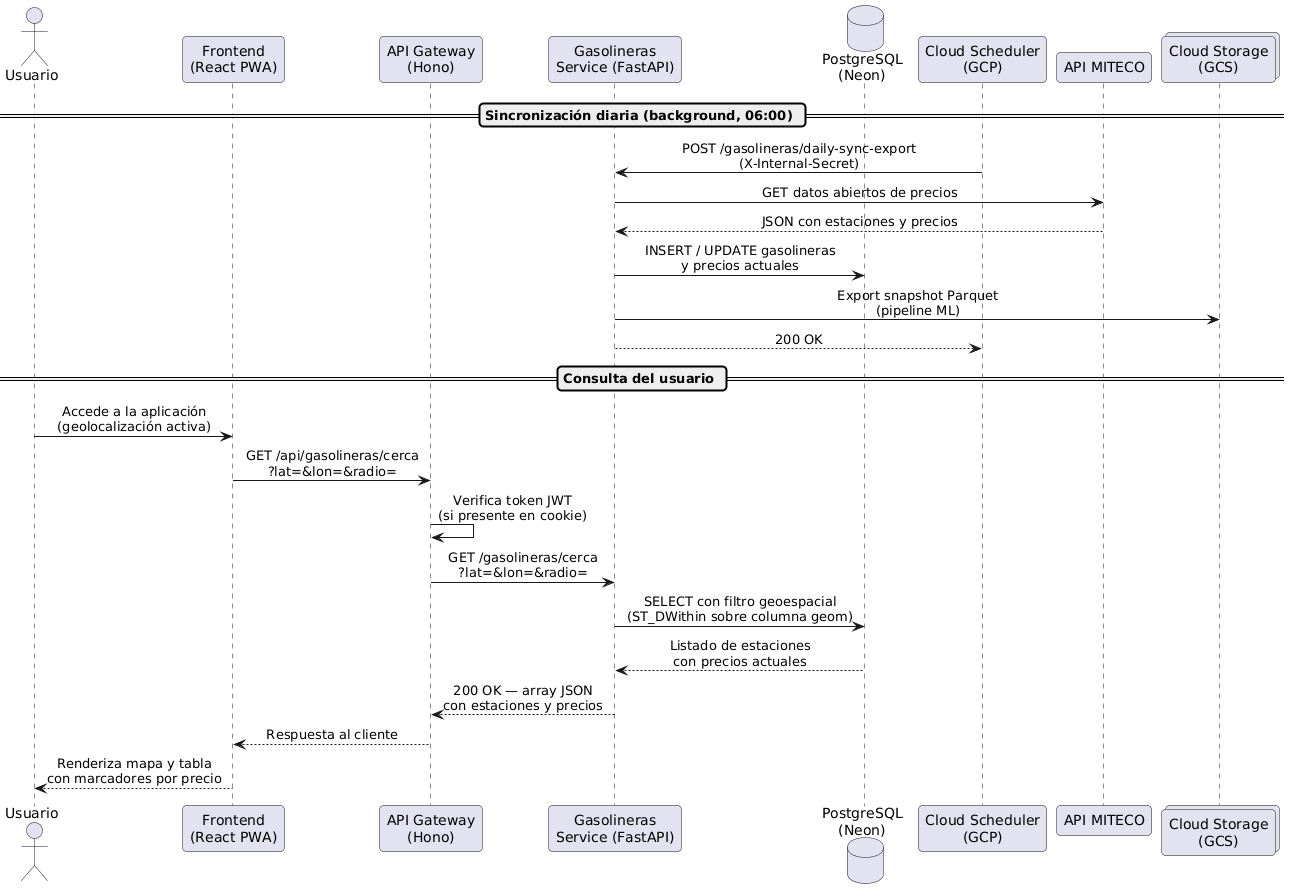
\includegraphics[width=0.85\textwidth]{imgs/secuencia-consulta.png}
  \caption{Diagrama de secuencia: consulta de gasolineras cercanas}
  \label{fig:secuencia_consulta}
\end{figure}

El segundo diagrama de secuencia, figura~\ref{fig:secuencia_ruta}, muestra el flujo de
planificación de ruta con recomendación de repostaje. El servicio de recomendación
coordina dos llamadas externas: a OpenRouteService para obtener el trazado de la ruta, y
al servicio de gasolineras para recuperar las estaciones cercanas al recorrido. Con ambas
respuestas aplica el algoritmo de ponderación por precio y desvío y devuelve las paradas
sugeridas al usuario.

\begin{figure}[H]
  \centering
  %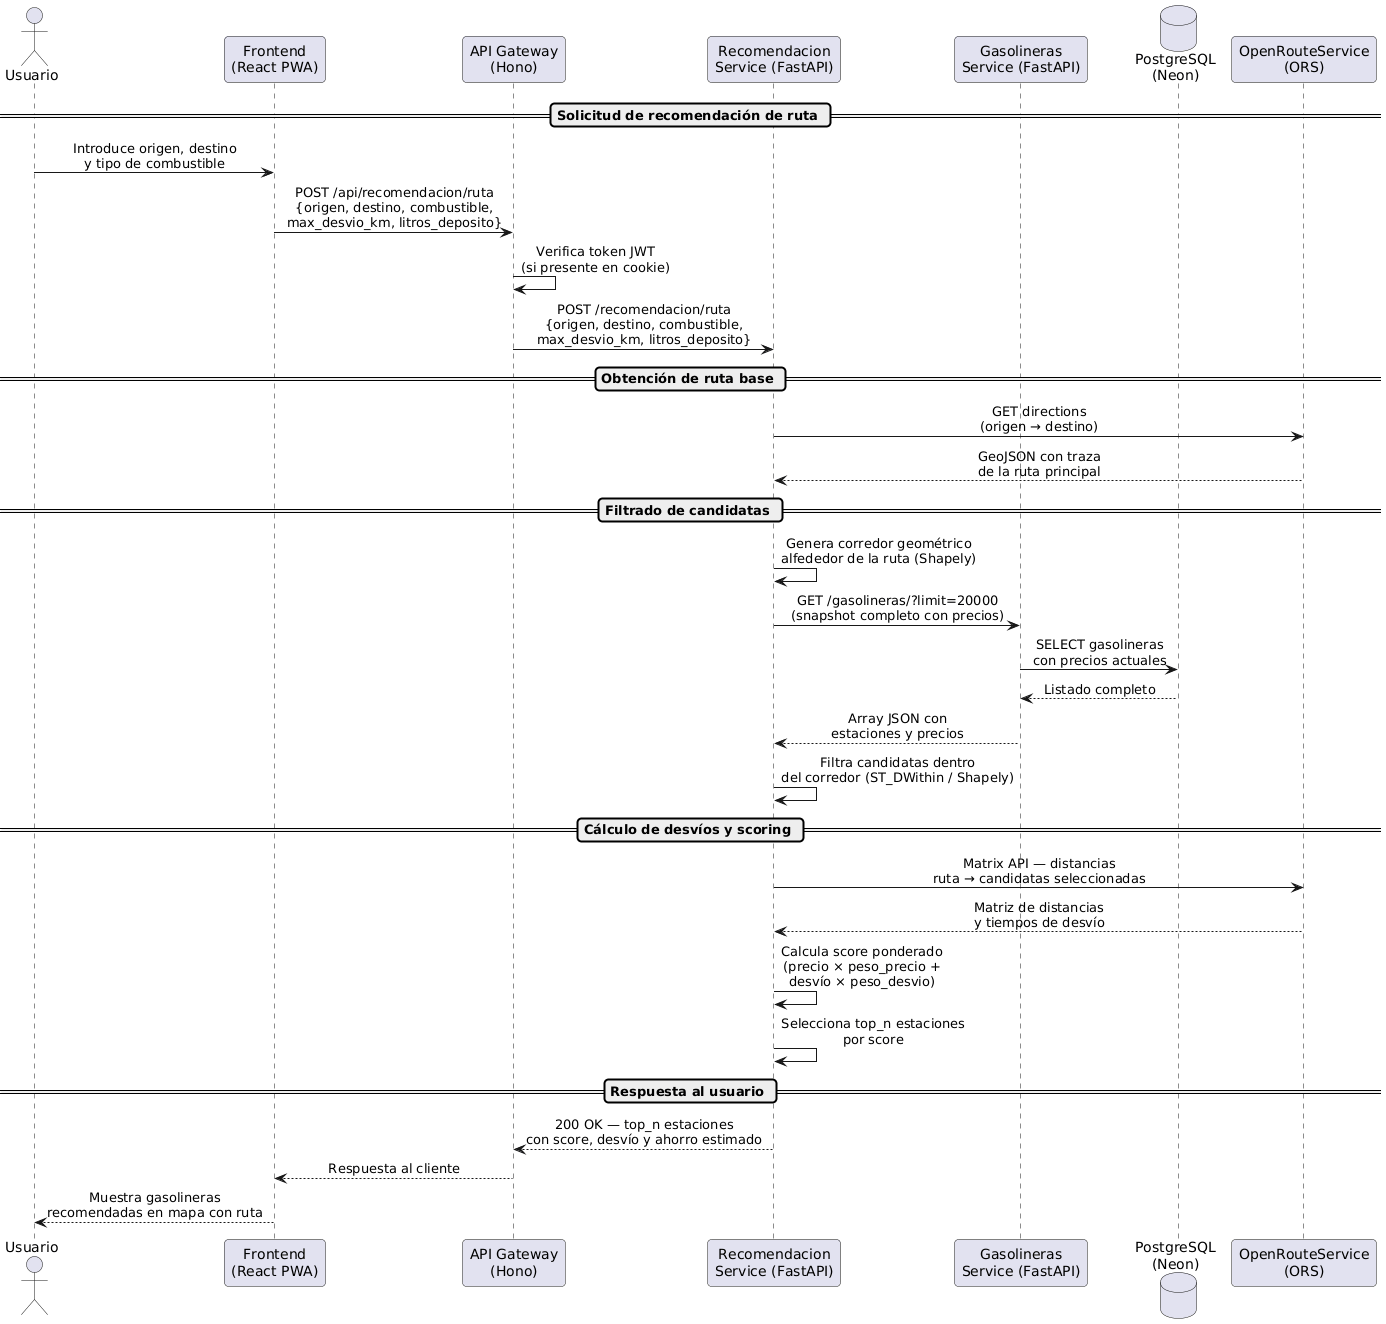
\includegraphics[width=0.85\textwidth]{imgs/secuencia-recomendacion.png}
  \caption{Diagrama de secuencia: planificación de ruta con recomendación de repostaje}
  \label{fig:secuencia_ruta}
\end{figure}

% ═════════════════════════════════════════════
\section{Consideraciones sobre la Implementación}
\label{sec:implementacion}
% ═════════════════════════════════════════════

Esta sección documenta las decisiones de implementación más relevantes de cada componente
del sistema, con especial atención a los aspectos que condicionan el comportamiento en
producción y que no quedan completamente cubiertos por la especificación de requisitos o el
diseño arquitectónico.

% ─────────────────────────────────────────────
\subsection{Estructura del proyecto}
\label{subsec:estructura}
% ─────────────────────────────────────────────

El repositorio sigue una estructura de monorepo, cada microservicio reside en su propio
directorio raíz y tiene su propio \texttt{Dockerfile}, su fichero de dependencias y su
conjunto de pruebas. Esta organización permite iterar sobre un servicio sin alterar el
resto y facilita la asignación de un pipeline de CI/CD independiente a cada componente.

Los directorios principales son \texttt{gateway-hono}, \texttt{gasolineras-service},
\texttt{usuarios-service}, \\
\texttt{recomendacion-service}, \texttt{prediction-service},
\texttt{voice-assistant-service}, \texttt{mcp-gasolineras-server} y
\texttt{frontend-client}. En la raíz se encuentran el \texttt{docker-compose.yml} para el
entorno local y los siete ficheros \texttt{cloudbuild-*.yaml} para el despliegue en
producción.

La orquestación local se basa en \textbf{Docker Compose}~\cite{docker_compose}, con
dependencias de arranque declaradas explícitamente, los servicios de dominio esperan a que
la base de datos esté accesible, el gateway espera a que los servicios de dominio superen
sus \textit{health checks}, el frontend arranca únicamente cuando el gateway está
disponible. Los servicios opcionales de IA y predicción se activan mediante perfiles Docker
(\texttt{ai}, \texttt{ml})~\cite{docker_compose_profiles}, de forma que la instalación base no requiere claves de API
externas.

% ─────────────────────────────────────────────
\subsection{Servicio de gasolineras y sincronización de datos}
\label{subsec:gasolineras_impl}
% ─────────────────────────────────────────────

El \texttt{gasolineras-service} es el componente con mayor complejidad operacional del
sistema, ya que combina la gestión de datos en tiempo real con la necesidad de mantener
frescura respecto a una fuente externa que actualiza sus precios varias veces al
día~\cite{datosgob_carburantes}.

\subsubsection*{Ciclo de sincronización}

El servicio implementa tres mecanismos de sincronización complementarios. En primer lugar,
al arrancar, si la variable \texttt{AUTO\_ENSURE\_FRESH\_ON\_STARTUP} está activa, el
servicio comprueba la antigüedad de los datos almacenados y lanza una sincronización
condicional si supera el umbral configurado. En segundo lugar, en producción un
\textbf{Cloud Scheduler} de Google Cloud Platform \cite{cloud_scheduler2026,gcp_products2026}
dispara diariamente un Cloud Run Job \cite{cloud_run2026} que invoca el endpoint interno 
\texttt{POST /gasolineras/daily-sync-export}, este endpoint
sincroniza los datos desde la API del Ministerio de Industria y, a continuación, exporta
un snapshot en formato Parquet a Google Cloud Storage \cite{cloud_storage2026} para el pipeline de machine learning.
En tercer lugar, si una petición de lectura detecta que los datos superan el umbral de
antigüedad (\texttt{AUTO\_SYNC\_ON\_READ=true}), el servicio puede desencadenar una
sincronización en segundo plano, aunque en producción esta opción se mantiene desactivada
para evitar latencia impredecible.

La combinación de estos mecanismos garantiza que los datos nunca superen 24 horas de
antigüedad en producción sin necesidad de un sistema de colas externo.

\subsubsection*{Almacenamiento y consultas geoespaciales}

Los precios actuales se almacenan en la tabla \texttt{gasolineras} junto con las
coordenadas geográficas de cada estación. Para las búsquedas por proximidad se utiliza
\textbf{PostGIS}~\cite{postgis}, la extensión geoespacial de PostgreSQL, que permite
ejecutar consultas basadas en distancia con los operadores \texttt{ST\_DWithin} y
\texttt{ST\_Distance} de forma eficiente mediante índices espaciales. Esto evita el
cálculo de la distancia haversine en capa de aplicación para el filtrado inicial,
reservándolo únicamente para el refinamiento de resultados.

El histórico de precios se registra en la tabla \texttt{precios\_historicos}, donde cada
fila representa una instantánea de los precios de una estación en una fecha concreta. Este
diseño permite construir series temporales por estación y combustible, que son la entrada
del modelo de predicción.

\subsubsection*{Fallback en memoria}

Si al arrancar el servicio no dispone de conexión a la base de datos, entra en modo
\textit{memory-fallback}: carga los datos desde la última sincronización disponible en
memoria y continúa respondiendo peticiones, aunque sin capacidad de escritura. Este modo
garantiza la resiliencia ante interrupciones transitorias de conectividad con Neon, que al
ser un servicio externo puede experimentar latencias de conexión en arranques en frío
(\textit{cold starts}) de Cloud Run.

\subsubsection*{Integración de electrolineras}

Los puntos de recarga eléctrica se obtienen de la API de Mapareve~\cite{mitma_esmovilidad}
y están integrados directamente dentro del \texttt{gasolineras-service}, bajo el prefijo
de rutas \texttt{/api/charging/}. Esta decisión evita la proliferación de microservicios
para funcionalidades que comparten el mismo patrón de acceso (consulta geoespacial, caché
corta) y reduce la complejidad operacional del despliegue.

% ─────────────────────────────────────────────
\subsection{Servicio de usuarios y autenticación}
\label{subsec:usuarios_impl}
% ─────────────────────────────────────────────

El \texttt{usuarios-service} gestiona el ciclo completo de identidad: registro,
autenticación tradicional, autenticación federada con Google OAuth y gestión de favoritos.
Está implementado con \textbf{Fastify}~\cite{fastify}, que en combinación con el plugin 
\texttt{@fastify/jwt}~\cite{fastify_jwt} proporciona la firma y verificación de tokens sin código boilerplate.

\subsubsection*{Autenticación y tokens JWT}

Tras un inicio de sesión correcto, el servicio genera un token \textbf{JWT}~\cite{jwt_rfc}
firmado con el algoritmo HS256 y una caducidad de 7 días. El token no se devuelve en el
cuerpo de la respuesta, sino que el API Gateway lo establece como una \textit{cookie}
\texttt{httpOnly} con los flags \texttt{Secure} y \texttt{SameSite=None} en producción.
Este mecanismo impide que el token sea accesible desde JavaScript del navegador, mitigando
ataques XSS~\cite{owasp_xss}.

Para el flujo de Google OAuth, el gateway actúa como intermediario: recibe el
\texttt{id\_token} de Google, lo verifica y llama al endpoint interno
\texttt{POST /api/usuarios/google/internal} con cabecera \texttt{X-Internal-Secret}, de
forma que este endpoint nunca queda expuesto al exterior. El servicio realiza un
\textit{upsert} del usuario (crea la cuenta si no existe, o la actualiza si ya existe por
email) y devuelve el JWT al gateway para su encapsulación en cookie.

Las contraseñas se almacenan únicamente como hash generado con \textbf{bcrypt}~\cite{bcrypt}
con 12 rondas de sal, lo que hace computacionalmente inviable su recuperación por fuerza
bruta incluso en caso de exfiltración de la base de datos.

\subsubsection*{Gestión del esquema de base de datos}

El proyecto no utiliza un sistema de migraciones automático tipo Flyway o Liquibase. El
esquema se define en un fichero \texttt{init.sql} con sentencias idempotentes
(\texttt{CREATE TABLE IF NOT EXISTS}, \texttt{ALTER TABLE IF NOT EXISTS}) que se aplican
manualmente sobre la instancia PostgreSQL de Neon en el primer despliegue. Esta decisión
es apropiada para el alcance del proyecto, aunque en un sistema de producción con múltiples
entornos sería recomendable introducir un gestor de migraciones formal para controlar la
evolución del esquema a lo largo del tiempo.

\subsubsection*{Rate limiting}

Los endpoints de registro e inicio de sesión aplican un límite de 5 peticiones por IP
cada 15 minutos mediante el plugin \texttt{@fastify/rate-limit}~\cite{fastify_ratelimit},
configurado con \texttt{global: false} para no afectar al resto de rutas. Las direcciones
de loopback (\texttt{127.0.0.1}, \texttt{::1}) quedan exentas para no interferir con las
pruebas locales.

% ─────────────────────────────────────────────
\subsection{Servicio de recomendación de ruta}
\label{subsec:recomendacion_impl}
% ─────────────────────────────────────────────

% Pendiente de desarrollar — el servicio de recomendación aún está en fase de refinamiento.

% ─────────────────────────────────────────────
\subsection{Módulo de predicción de precios}
\label{subsec:prediccion_impl}
% ─────────────────────────────────────────────

El \texttt{prediction-service} implementa un pipeline de machine learning para estimar el
precio de combustible de las estaciones favoritas de los usuarios durante los próximos 7
días. El diseño se orienta a la ejecución periódica en lote (\textit{batch}) más que a la
inferencia en tiempo real.

\subsubsection*{Selección del modelo}

Se evaluaron varios enfoques de regresión para series temporales: modelos ARIMA clásicos,
redes LSTM y árboles potenciados por gradiente. Se ha optado por \textbf{LightGBM}~\cite{lgbm}
en régimen de \textbf{regresión cuantílica} por tres razones principales. Primero, ofrece
un rendimiento muy competitivo en tablas de series temporales con features derivadas sin
requerir la normalización y el ajuste de hiperparámetros extensivo que exigen las redes
neuronales recurrentes. Segundo, la regresión cuantílica (cuantiles 0.05, 0.50, 0.95)
produce directamente intervalos de confianza para cada predicción, lo que enriquece la
información presentada al usuario. Tercero, LightGBM tiene un tiempo de entrenamiento muy
reducido, compatible con la ejecución semanal del job en un entorno serverless con límites
de memoria y CPU~\cite{ke2017lightgbm}.

\begin{figure}[H]
  \centering
  %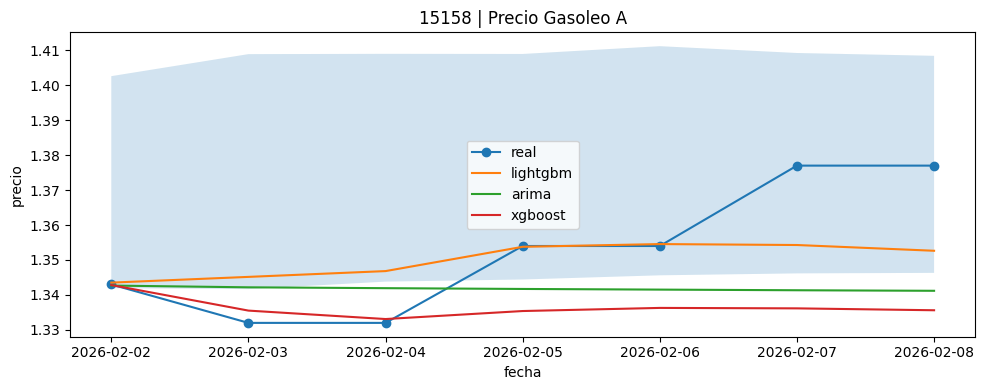
\includegraphics[width=0.85\textwidth]{imgs/prediccion_mae_comparativa.png}
  \caption{Comparativa de MAE entre modelos evaluados durante el desarrollo}
  \label{fig:mae_comparativa}
\end{figure}

\subsubsection*{Ingeniería de \textit{features}}

Para cada estación y tipo de combustible se construye una serie temporal diaria con el
precio medio registrado. A partir de ella se generan \textit{features} temporales
(día de la semana, fin de semana, semana del año, mes, trimestre), \textit{lags} de 1, 7,
14, 21 y 30 días, medias móviles y desviaciones típicas de ventanas de 7, 14 y 30 días,
y diferencias a 1 y 7 días. Adicionalmente, si la conexión a internet está disponible,
se descarga el precio del crudo Brent mediante \textbf{yfinance}~\cite{yfinance} y se
incorporan sus lags como variable exógena, aprovechando la correlación conocida entre el
precio del petróleo y los precios en surtidor~\cite{LAHMIRI2024105008}.

\subsubsection*{Ciclo de entrenamiento e inferencia}

El pipeline se ejecuta semanalmente mediante un \textbf{Cloud Run Job} disparado por
\textbf{Cloud Scheduler} (cada lunes a las 06:00 UTC). En cada ejecución, el job descarga
los snapshots Parquet de los últimos 180 días desde Google Cloud Storage, valida que los
datos estén frescos, reentrena el modelo para cada par (estación, combustible), genera
las predicciones de los 7 días siguientes de forma secuencial —cada día nuevo utiliza las
predicciones previas para recalcular los lags— y persiste los resultados en la tabla
\texttt{prediction\_forecasts} de PostgreSQL. Los artefactos del modelo entrenado
(\texttt{.pkl}) se almacenan en el bucket GCS bajo el prefijo \texttt{modelos\_lgbm/}
para su eventual reutilización.

La selección de estaciones a predecir se basa en los favoritos globales de los usuarios:
el job consulta el endpoint interno \texttt{/api/usuarios/favoritos/all-ideess} para
obtener los identificadores únicos de las estaciones con al menos un usuario que las ha
marcado como favoritas. Este criterio concentra la capacidad de cómputo en las estaciones
con mayor demanda real, evitando el coste prohibitivo de entrenar modelos para las más
de 11\,000 estaciones del catálogo nacional.

\subsubsection*{Consulta de predicciones}

En producción el servicio opera en modo API (\texttt{RUN\_HTTP\_API=true}): no ejecuta el
pipeline de entrenamiento, sino que expone el endpoint
\texttt{GET /api/prediction/station/\{ideess\}} que lee directamente de la tabla
\texttt{prediction\_forecasts}. El entrenamiento y la escritura en base de datos son
responsabilidad exclusiva del Cloud Run Job periódico, separando claramente los roles de
escritura y lectura.

% ─────────────────────────────────────────────
\subsection{Asistente conversacional de voz}
\label{subsec:voice_impl}
% ─────────────────────────────────────────────

El \texttt{voice-assistant-service} implementa un asistente de dominio restringido que
permite al usuario realizar consultas sobre gasolineras en lenguaje natural, tanto por
texto como por voz, y recibir una respuesta en audio. El servicio está implementado con
\textbf{Fastify}~\cite{fastify} y se integra con la API de \textbf{Google Gemini}~\cite{gemini}
mediante llamadas HTTP REST al cliente \texttt{@google/genai}.

\subsubsection*{Pipeline STT $\rightarrow$ LLM $\rightarrow$ TTS}

El pipeline se ejecuta en tres etapas secuenciales, cada una con su propia llamada a la
API de Gemini. En la etapa de \textbf{reconocimiento de voz} (\textit{Speech-to-Text}),
si la petición incluye audio en base64, el servicio invoca \texttt{generateContent} con
el modelo configurado para transcribir el audio a texto. En la etapa de \textbf{razonamiento}
(\textit{LLM con function calling}), se realiza una primera llamada con las declaraciones
de las funciones disponibles (\texttt{get\_prices} y \texttt{get\_nearest\_stations}); si
el modelo solicita ejecutar alguna de ellas, el servicio las invoca localmente contra el
API Gateway y realiza una segunda llamada con los resultados, obteniendo así la respuesta
final fundamentada en datos reales. En la etapa de \textbf{síntesis de voz}
(\textit{Text-to-Speech}), se realiza una llamada adicional a Gemini con modalidad de
respuesta \texttt{AUDIO}, la respuesta PCM se convierte a WAV y se devuelve en base64
al cliente.

Este diseño con tres llamadas separadas, en lugar de una única llamada multimodal, ofrece
mayor control sobre cada etapa y facilita el manejo de errores y los fallbacks por modelo.

\subsubsection*{Guardarraíles y control del dominio}

Dado que el asistente está diseñado para un dominio muy específico, se implementan varios
mecanismos para evitar un uso fuera de ámbito. Un \textbf{comprobador de alcance}
(\textit{scope guard}) basado en palabras clave evalúa la transcripción antes de invocar
el LLM; si la consulta no contiene términos relacionados con combustible, gasolineras,
precios o navegación, y la variable \texttt{VOICE\_GUARDRAILS\_ENABLED} está activa, el
servicio devuelve una respuesta predefinida sin consumir tokens del modelo. El modo
\texttt{strict} rechaza directamente la petición; el modo \texttt{soft} permite continuar
con una advertencia al modelo.

Adicionalmente, el \textbf{system prompt} construido por \texttt{buildSystemInstruction}
instruye explícitamente al modelo sobre el idioma, el tono y el formato esperados, y lo
obliga a utilizar las funciones declaradas para cualquier consulta de datos, reduciendo el
riesgo de alucinaciones. El function calling se ejecuta en el servidor, de forma que el
LLM nunca interactúa directamente con el gateway, sino que proporciona los parámetros de
la llamada y espera los resultados.

Otros controles operativos incluyen límites de tamaño de payload
(\texttt{VOICE\_MAX\_TEXT\_CHARS}, \texttt{VOICE\_MAX\_AUDIO\_BASE64\_CHARS}), timeouts
por llamada a Gemini con \texttt{AbortController}, y rate limiting por IP para el
transporte WebSocket. Como limitación conocida, el rate limiter no se aplica actualmente
al endpoint HTTP \texttt{/voice/dialog}, aspecto identificado para una iteración futura.

\subsubsection*{Nota sobre el transporte WebSocket}

El servicio implementa tanto el endpoint HTTP \texttt{POST /voice/dialog} como un
endpoint WebSocket \texttt{/ws/voice} para streaming de audio. Durante el desarrollo se
identificaron problemas de estabilidad de conexión con el transporte WebSocket en el
entorno de Cloud Run, asociados al comportamiento de las peticiones de larga duración en
infraestructura serverless. Por ello, el cliente frontend utiliza actualmente el endpoint
HTTP, que ofrece un comportamiento predecible en todos los entornos de despliegue.

% ─────────────────────────────────────────────
\subsection{Frontend: React PWA con Nginx}
\label{subsec:frontend_impl}
% ─────────────────────────────────────────────

El frontend es una \textit{Single Page Application} (SPA) construida con
\textbf{React 19}~\cite{react} y \textbf{TypeScript}~\cite{typescript}, compilada con
\textbf{Vite}~\cite{vite} y empaquetada como \textbf{Progressive Web App}
(PWA)~\cite{pwa_spec}. En producción, los artefactos estáticos generados por Vite se
sirven mediante \textbf{Nginx}~\cite{nginx} dentro de un contenedor Docker de imagen
mínima.

\subsubsection*{Configuración de Nginx}

Nginx está configurado para servir el directorio \texttt{dist} generado por Vite desde
\texttt{/usr/share/nginx/html}. La directiva \texttt{try\_files \$uri \$uri/ /index.html}
garantiza que todas las rutas no estáticas sean resueltas por el router de React en
cliente, comportamiento necesario para el correcto funcionamiento de la navegación SPA.
Los assets estáticos con huella de contenido (\texttt{.js}, \texttt{.css}, fuentes e
imágenes) se cachean durante un año con la cabecera
\texttt{Cache-Control: public, immutable}, lo que maximiza el rendimiento en visitas
recurrentes. Nginx no actúa como proxy inverso para la API en producción: todas las
llamadas al backend se dirigen directamente a la URL del API Gateway configurada en
tiempo de compilación mediante la variable \texttt{VITE\_API\_BASE\_URL}.

\subsubsection*{Progressive Web App}

La aplicación implementa el estándar PWA mediante el plugin
\textbf{vite-plugin-pwa}~\cite{vite_pwa} con Workbox~\cite{workbox} como gestor del
Service Worker. El fichero \texttt{manifest.webmanifest} define los metadatos necesarios
para la instalación en dispositivos móviles (nombre, iconos, color de tema y modo de
visualización \textit{standalone}). El Service Worker implementa una estrategia de caché
que permite el acceso a la interfaz aunque la conexión sea intermitente, aunque las
consultas de datos en tiempo real requieren conectividad activa.

\subsubsection*{Internacionalización y diseño responsivo}

La interfaz soporta tres idiomas (español, inglés y euskera) mediante
\textbf{i18next}~\cite{i18next} con detección automática del idioma del navegador. El
diseño sigue un enfoque \textit{mobile-first} con \textbf{TailwindCSS}~\cite{tailwind},
garantizando que la experiencia sea funcional tanto en pantallas de escritorio como en
dispositivos móviles, donde el caso de uso de búsqueda de gasolineras en ruta es
predominante. El mapa interactivo se implementa con \textbf{Leaflet}~\cite{leaflet} a
través de la librería \texttt{react-leaflet}, con soporte para clustering de marcadores
a niveles de zoom bajos para evitar la saturación visual cuando hay muchas estaciones en
el área visible.

% ─────────────────────────────────────────────
\subsection{Despliegue en GCP y pipeline CI/CD}
\label{subsec:despliegue_impl}
% ─────────────────────────────────────────────

Todos los microservicios se despliegan en \textbf{Google Cloud Run}~\cite{cloud_run},
plataforma serverless que gestiona el escalado automático en función de la demanda y
factura únicamente por el tiempo de cómputo efectivo. Esta elección elimina la necesidad
de gestionar instancias o clústeres, lo que reduce significativamente la carga operacional
para un proyecto académico sin comprometer la disponibilidad.

\subsubsection*{Pipeline de CI/CD}

Cada microservicio dispone de su propio fichero \texttt{cloudbuild-*.yaml} que define un
pipeline de \textbf{Cloud Build}~\cite{cloud_build} independiente. Los pipelines se
activan automáticamente con cada \textit{push} a la rama \texttt{main} del repositorio.
El proceso consta de tres pasos: construcción de la imagen Docker, publicación en
\textbf{Artifact Registry}~\cite{artifact_registry} (región \texttt{europe-west1}), y
despliegue en Cloud Run con las variables de entorno inyectadas desde
\textbf{Secret Manager}~\cite{secret_manager}. Este diseño garantiza que ningún secreto
esté presente en el repositorio ni en los logs de compilación.

El pipeline del frontend incluye validaciones adicionales en el paso de compilación: la
variable \texttt{VITE\_API\_BASE\_URL} debe apuntar a un dominio HTTPS (no a
\texttt{localhost}), lo que previene despliegues accidentales de configuraciones de
desarrollo.

\subsubsection*{Comunicación entre servicios en Cloud Run}

En Cloud Run cada servicio tiene una URL pública asignada por Google, pero la comunicación
interna entre servicios no debe transitar por internet. Para ello, el gateway utiliza
tokens IAM de servicio (\textit{service account tokens}) inyectados mediante el módulo
\texttt{cloudRunAuthFetch.js}, que autentica cada llamada inter-servicio ante la
infraestructura de Google sin exponer los servicios internos a peticiones externas no
autorizadas.

\subsubsection*{Base de datos y almacenamiento}

La base de datos PostgreSQL reside en \textbf{Neon Tech}~\cite{neon}, proveedor de
PostgreSQL serverless que ofrece \textit{branching} de bases de datos, hibernación
automática de instancias inactivas y conexión mediante cadena estándar
\texttt{postgresql://}. La elección de un proveedor externo en lugar de Cloud SQL de GCP
responde a la disponibilidad de un plan gratuito suficiente para las cargas del proyecto
y a la independencia del proveedor cloud para la capa de datos.

Los snapshots Parquet del pipeline de ML y los modelos entrenados se almacenan en
\textbf{Google Cloud Storage}~\cite{gcs}, que actúa como capa de almacenamiento de objetos
entre el servicio de gasolineras (productor de datos), el job de predicción (consumidor y
productor de modelos) y el servicio de predicción en modo API (lector de resultados).

% ─────────────────────────────────────────────
\subsection{Seguridad transversal}
\label{subsec:seguridad_impl}
% ─────────────────────────────────────────────

Además de los mecanismos de autenticación descritos en la sección anterior, el sistema
implementa un conjunto de controles de seguridad aplicados de forma transversal.

La comunicación entre el gateway y los microservicios internos está protegida por la
cabecera \texttt{X-Internal-Secret}: los endpoints de administración (sincronización
forzada, export, consulta de favoritos globales) rechazan con \texttt{403 Forbidden}
cualquier petición que no incluya el secreto configurado en \texttt{INTERNAL\_API\_SECRET}.
Este mecanismo evita que dichos endpoints sean accesibles desde el exterior incluso si
un servicio queda expuesto inadvertidamente.

La validación de datos de entrada se realiza en capa de aplicación con
\textbf{Pydantic v2}~\cite{pydantic} en los servicios Python y con los esquemas de
validación de Fastify en los servicios Node.js. Los parámetros de consulta con potencial
de abuso (radio de búsqueda, límite de resultados) tienen cotas máximas declaradas
explícitamente. Las consultas a PostgreSQL utilizan siempre parámetros preparados, sin
concatenación de cadenas, eliminando el vector de inyección SQL~\cite{owasp_sqli}.

El servicio de usuarios aplica \textbf{Helmet.js}~\cite{helmetjs} para establecer
cabeceras HTTP de seguridad (\texttt{X-Frame-Options}, \texttt{Content-Security-Policy},
\texttt{X-Content-Type-Options}). En producción, Cloud Run gestiona HTTPS
automáticamente, de forma que todo el tráfico externo está cifrado en tránsito. Los
secretos de producción (claves de API, cadenas de conexión, JWT secret) nunca residen en
el repositorio y se inyectan en tiempo de ejecución desde Secret Manager.
\section{Plan de Pruebas}
\subsection{Estrategia}
\subsection{Pruebas unitarias}
\subsection{Pruebas de integración}
\subsection{Pruebas funcionales}
\subsection{Resultados obtenidos}

\section{Manual de Usuario}
\subsection{Acceso al sistema}
\subsection{Uso de la plataforma}
\subsection{Capturas de pantalla}

\section{Incidencias del Proyecto}
